%% how_turkic_is_anatolian_turkish: short paper. First version 2026-10-29 (old_versions/main_2026-10-29_first_version.tex);
%% second version 2026-10-30, rebuilt on the Hanami DNA reference data and the author's Illustrative DNA results.
%% Sources: ../models/core-anatolia.md, ../results/*.json (from ../analysis/), ../data/samples.md, ../bibliography.bib.
%% figures/regions.tex, closeness.tex and pca.tex are generated by ../analysis/10_paper_figures.py; do not edit them by hand.
\documentclass[conference,a4paper]{IEEEtran}
\usepackage[T1]{fontenc}
\usepackage[utf8]{inputenc}
\usepackage{microtype,booktabs,amsmath,array}
\usepackage{tikz}
\usetikzlibrary{arrows.meta,positioning,calc,patterns,decorations.pathreplacing}
\usepackage{cite}
\usepackage[hidelinks]{hyperref}

% Okabe--Ito palette (colour-blind safe); every figure also uses a pattern or label so it reads in greyscale.
\definecolor{tkblue}{HTML}{0072B2}
\definecolor{tkverm}{HTML}{D55E00}
\definecolor{tkgreen}{HTML}{009E73}
\definecolor{tkorange}{HTML}{E69F00}
\definecolor{tksky}{HTML}{56B4E9}
\definecolor{tkink}{HTML}{2B2B2B}

\title{How Turkic Is Anatolian Turkish?}

\author{\IEEEauthorblockN{Umay~\c{S}aml\i{}}
\IEEEauthorblockA{\textit{Independent researcher}\\
samliumay965@gmail.com}}

\begin{document}
\bstctlcite{IEEEexample:BSTcontrol}
\maketitle

\begin{abstract}
How much of the modern Anatolian Turkish genome comes from the medieval Turkic populations of the steppe, and how much from the people who already lived in Anatolia when the Seljuks arrived? We model modern Turkish regional averages from the published Global-25 (G25) reference data as mixtures of Byzantine Anatolia (AD 500--1100), a medieval Turkic pool from Kazakhstan and Kyrgyzstan (AD 650--1200) and a Kartvelian source. The core of Anatolia (778 people from the western, central and northern provinces) fits as 54.9\% Byzantine Anatolia, 23.1\% medieval Turkic and 21.9\% Kartvelian, and the core regions range from 20.6\% to 28.2\% Turkic. The author's own kit gives 23.0\% on a commercial model. Replacing the steppe pool with the Çapalıbağ individuals of southwestern Türkiye (1300--1650 CE), the earliest Anatolian Turks with published DNA, improves every core fit. The core regions come out 56.9\% to 77.2\% Çapalıbağ-like, and an Ottoman-era source from Kaman-Kalehöyük gives the same Turkic share by a third route. An appendix fits all three models to 89 Turkish subgroups. Splitting the pre-Turkic side shows a Bronze Age Anatolian and Caucasian base with no Greek component. The closest modern populations to core Anatolia are Azerbaijanis, followed by western and Alevi Kurds and eastern Turks who share the Azerbaijani cluster; Greeks are no closer than Armenians, and the non-Oghuz Turkic peoples of Central Asia are distant.
\end{abstract}

\begin{IEEEkeywords}
ancient DNA, admixture modeling, Global-25, Anatolia, Turkic peoples, Göktürk Khaganate, Seljuks, Çapalıbağ
\end{IEEEkeywords}

\section{Introduction}
Few questions start more arguments online in Türkiye than ``how Turkic are the Turks?'' Most answers are ideological. A narrower version of the question can be answered with genetics: what share of the modern Anatolian genome traces back to the medieval Turkic populations of the steppe, and what share to the population that was already in Anatolia when the Seljuks arrived after 1071?

We answer it with G25 principal-component coordinates and published ancient DNA, in four steps. Section~\ref{sec:anchor} explains why the Turkic source starts at the Göktürk era. Section~\ref{sec:data} describes the sources and the two control sites, and Section~\ref{sec:method} the fitting. Section~\ref{sec:results} reports the fits for every Turkish region, what the pre-Turkic layer is made of, and where modern Anatolian Turks sit among other populations. The analysis scripts, the model definitions and the results are in the project repository.\footnote{\url{https://github.com/samliumay/how_turkic_is_anatolian_turkish}}

\section{What ``Turkic'' Means in the Model}\label{sec:anchor}
``Turkic'' has no single genetic origin, and the record gets less certain the further back it goes. The first Turkic-speaking peoples attested in written sources are the Oghur-speaking tribes on the Pontic steppe in the 5th century CE. The first people to call themselves \textit{Türk} are those of the Göktürk Khaganate, founded in 552. Before that, the names belong to confederations whose make-up is debated. The language or languages of the Xiongnu may have been Turkic, Mongolic, Yeniseian or a mixture, and the European Huns are just as unresolved. These confederations were political units, not genetic ones. There is therefore no clean proto-Turkic population to fit against, and we do not try.

The Göktürks are a usable anchor. They are the first identifiable Turkic polity, and the medieval Turkic individuals of the Central Steppe and the Tian Shan represent their population genetically~\cite{damgaard2018steppes,jeong2020}. These individuals were already mixed: they sit between ancient West Eurasian and East Eurasian populations. In this paper ``Turkic'' therefore means that Göktürk-era profile of AD 650--1200, not a pure steppe origin. After the Western Turkic Khaganate fell in the 7th century, the Oghuz moved west, and their descendants, the Seljuks, entered Anatolia after the battle of Manzikert in 1071 (Fig.~\ref{fig:timeline}).

\begin{figure}[t]
\centering
% Timeline of sources, controls and anchor events (AD 400--2000). x: 1 cm = 200 years, origin at AD 400.
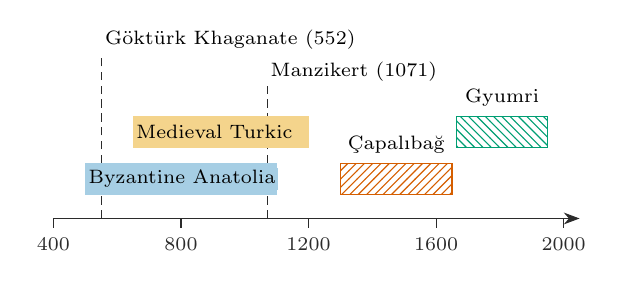
\begin{tikzpicture}[x=0.0405mm, y=1mm, font=\scriptsize]
  \def\yr#1{(#1-400)}
  % axis
  \draw[tkink, -{Stealth[length=2mm]}] (0,0) -- (1650,0);
  \foreach \t in {400,800,1200,1600,2000}
    \draw[tkink] ({\t-400},0) -- ({\t-400},-1.2) node[below] {\t};
  % anchor events
  \foreach \t/\lab/\h in {552/Göktürk Khaganate (552)/21, 1071/Manzikert (1071)/17} {
    \draw[tkink, densely dashed] ({\t-400},0) -- ({\t-400},\h);
    \node[anchor=south west, inner sep=1pt] at ({\t-400},\h) {\lab};
  }
  % source windows (shaded), drawn over the event lines

  \fill[tkblue!35] ({500-400},3) rectangle ({1100-400},7);
  \node[anchor=west, fill=tkblue!35, inner sep=1pt] at ({500-400},5) {Byzantine Anatolia};
  \fill[tkorange!45] ({650-400},9) rectangle ({1200-400},13);
  \node[anchor=west, fill=tkorange!45, inner sep=1pt] at ({650-400},11) {Medieval Turkic};
  % control sites (hatched)
  \fill[pattern=north east lines, pattern color=tkverm] ({1300-400},3) rectangle ({1650-400},7);
  \draw[tkverm] ({1300-400},3) rectangle ({1650-400},7);
  \node[anchor=south] at ({1475-400},7) {Çapalıbağ};
  \fill[pattern=north west lines, pattern color=tkgreen] ({1665-400},9) rectangle ({1950-400},13);
  \draw[tkgreen] ({1665-400},9) rectangle ({1950-400},13);
  \node[anchor=south] at ({1807-400},13) {Gyumri};
\end{tikzpicture}

\caption{Model sources and controls on a timeline. Shaded bands are the date windows of the two ancient sources; hatched bands are the two control sites from \cite{lazaridis2022}. Vertical marks are the attested events used to anchor the Turkic source.}
\label{fig:timeline}
\end{figure}

\section{Data}\label{sec:data}
\subsection{Reference data and targets}
All population averages come from the published G25 reference data as used by Hanami DNA: 3,227 modern and 5,071 ancient rows. A group average weights each row by its sample size and leaves out outlier, low-resolution and contaminated rows. The targets are Turkish regional averages: West Anatolia (229 people), Central Anatolia (387), North Anatolia along the western Black Sea (175), the south around Adana, Mersin and Gaziantep (109), Trabzon, Rize and Artvin (48), Erzurum and the east (75) and the Balkan Turks (57). Core Anatolia is the first three together (778 people, including Istanbul's Anatolian-profile rows). For comparison we fit the Caucasus Azerbaijani average (134).

\subsection{Sources}
Table~\ref{tab:sources} lists the sources. The medieval Turkic pool holds the Early Medieval Turk, Karakhanid and Kipchak individuals from Kazakhstan and Kyrgyzstan~\cite{damgaard2018steppes,damgaard2018horse}. Byzantine Anatolia is the pre-Seljuk baseline. The Kartvelian source stands for the Caucasus-side component.

\begin{table}[t]
\centering
\caption{Sources of the medieval models}
\label{tab:sources}
\small
\begin{tabular}{@{}>{\raggedright}p{0.25\columnwidth}>{\raggedright}p{0.2\columnwidth}>{\raggedright\arraybackslash}p{0.45\columnwidth}@{}}
\toprule
Source & Period & Rows \\
\midrule
Medieval Turkic & AD 650--1200 & Kazakhstan and Kyrgyzstan Early Medieval Turk, Karakhanid, Kipchak (8 people) \\
Byzantine Anatolia & AD 500--1100 & Nicaea, Barcın, Ilıpınar, Samantas, Stratonikeia (26 people) \\
Early Anatolian Turkic & 1300--1650 & Çapalıbağ, SW Türkiye (12 people) \\
Ottoman Anatolian Turkic & Early Modern & Kaman-Kalehöyük, central Anatolia (3 people) \\
Kartvelian & modern & Georgian, Mingrelian, Svan, Laz \\
\bottomrule
\end{tabular}
\end{table}

\subsection{Controls}
Two sites from the Southern Arc study~\cite{lazaridis2022} anchor the migration in time.

\textit{Çapalıbağ, southwestern Türkiye (1300--1650 CE).} These individuals postdate the establishment of the Seljuk dynasty and carry substantial East Asian ancestry. The Y-chromosome lines include N-A9416, a Northeast Asian paternal line, and the mitochondrial lines include the East Eurasian A17 next to West Eurasian lines (W9, K1b1c, H13a1a1, HV14a, T2a1a, J2b2, H43, K1a). Their dates fall roughly 12 generations after the Seljuk expansion, and they sit halfway between Byzantine Anatolians and their Central Asian ancestors. They were descendants of real migrants who had already mixed with the local population. On our sources Çapalıbağ models as 47.3\% Byzantine Anatolia, 36.7\% medieval Turkic and 16.0\% Kartvelian (fit 1.17), so we also use it as an early Anatolian Turkic source.

\textit{Kaman-Kalehöyük, central Anatolia (Early Modern).} Three Ottoman-era individuals with Turkish and Turkic profiles. They model as 61.1\% medieval Turkic, 27.3\% Byzantine Anatolia and 11.6\% Kartvelian (fit 1.74). With only three people, we use them as a second, later Anatolian Turkic source and read their results as a cross-check.

\textit{Gyumri, Black Fortress cemetery, Armenia (1665--1950 CE).} One post-medieval individual, I18247, has a profile similar to present-day Azerbaijanis, unlike the Late Bronze Age individuals from the same site. It shows the Azerbaijani-like Oghuz profile in the Caucasus centuries ago.

\section{Method}\label{sec:method}
Each population is represented by its 25 scaled G25 coordinates. A target is modeled as a mixture of sources with non-negative weights that sum to one, chosen to minimize the Euclidean distance between the target and the mixture. The fit distance is that remaining distance times 100. Smaller is better, and it is only comparable between runs on the same coordinates. Distances between populations use the same scale. We fit three models to every target. Each combines Byzantine Anatolia and Kartvelian with one Turkic source: the medieval Turkic pool, Çapalıbağ, or Kaman-Kalehöyük. To split the pre-Turkic side, we fit the core average to Bronze Age Anatolia (EBA to MLBA), Mycenaean Greeks, La Tène Celts as a Galatian proxy, the Late Bronze Age Caucasus (Armenia) and the medieval Turkic pool, and repeat the fit over six source sets. The principal component analysis (PCA) is computed on 389 modern rows; ancient groups and the author are projected onto it.

\section{Results}\label{sec:results}
\subsection{The author's kit}
Fig.~\ref{fig:periods} shows the author's kit on Illustrative DNA, one model per period. In the medieval model the kit is 56.2\% Byzantine Anatolia, 23.0\% Turkic, 18.8\% Kartvelian and 2.0\% Iranian Plateau (fit 1.779). In every earlier period the local Anatolian layer is about a third (35.8\% to 36.4\%), and the Caucasus and Iranian side is a quarter to a third.

\begin{figure}[t]
\centering
% The author's kit on Illustrative DNA, one model per period (read 2026-10-30).
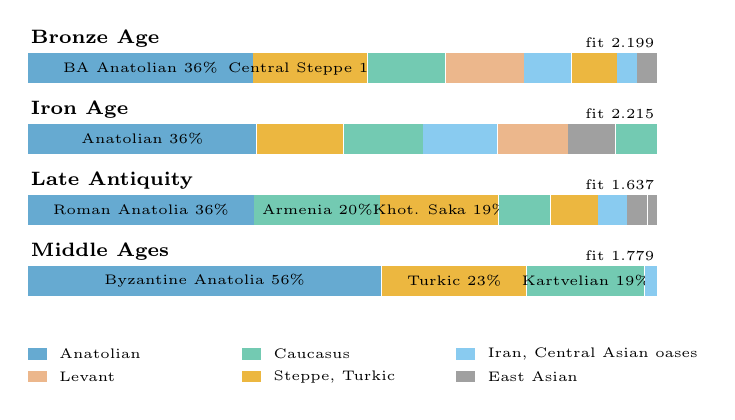
\begin{tikzpicture}[x=0.8mm, y=-9mm, font=\tiny]
  \node[anchor=south west, font=\scriptsize\bfseries, inner sep=1pt] at (0,0-0.28) {Bronze Age};
  \node[anchor=south east, inner sep=1pt] at (100,0-0.28) {fit 2.199};
  \fill[tkblue!60] (0.0,0-0.25) rectangle (35.8,0+0.18);
  \draw[white, line width=0.4pt] (35.8,0-0.25) -- (35.8,0+0.18);
  \node at (17.9,0-0.035) {BA Anatolian 36\%};
  \fill[tkorange!75] (35.8,0-0.25) rectangle (54.0,0+0.18);
  \draw[white, line width=0.4pt] (54.0,0-0.25) -- (54.0,0+0.18);
  \node at (44.9,0-0.035) {Central Steppe 18\%};
  \fill[tkgreen!55] (54.0,0-0.25) rectangle (66.4,0+0.18);
  \draw[white, line width=0.4pt] (66.4,0-0.25) -- (66.4,0+0.18);
  \fill[tkverm!45] (66.4,0-0.25) rectangle (78.8,0+0.18);
  \draw[white, line width=0.4pt] (78.8,0-0.25) -- (78.8,0+0.18);
  \fill[tksky!70] (78.8,0-0.25) rectangle (86.4,0+0.18);
  \draw[white, line width=0.4pt] (86.4,0-0.25) -- (86.4,0+0.18);
  \fill[tkorange!75] (86.4,0-0.25) rectangle (93.6,0+0.18);
  \draw[white, line width=0.4pt] (93.6,0-0.25) -- (93.6,0+0.18);
  \fill[tksky!70] (93.6,0-0.25) rectangle (96.8,0+0.18);
  \draw[white, line width=0.4pt] (96.8,0-0.25) -- (96.8,0+0.18);
  \fill[tkink!45] (96.8,0-0.25) rectangle (100.0,0+0.18);
  \draw[white, line width=0.4pt] (100.0,0-0.25) -- (100.0,0+0.18);
  \node[anchor=south west, font=\scriptsize\bfseries, inner sep=1pt] at (0,1-0.28) {Iron Age};
  \node[anchor=south east, inner sep=1pt] at (100,1-0.28) {fit 2.215};
  \fill[tkblue!60] (0.0,1-0.25) rectangle (36.4,1+0.18);
  \draw[white, line width=0.4pt] (36.4,1-0.25) -- (36.4,1+0.18);
  \node at (18.2,1-0.035) {Anatolian 36\%};
  \fill[tkorange!75] (36.4,1-0.25) rectangle (50.2,1+0.18);
  \draw[white, line width=0.4pt] (50.2,1-0.25) -- (50.2,1+0.18);
  \fill[tkgreen!55] (50.2,1-0.25) rectangle (62.8,1+0.18);
  \draw[white, line width=0.4pt] (62.8,1-0.25) -- (62.8,1+0.18);
  \fill[tksky!70] (62.8,1-0.25) rectangle (74.6,1+0.18);
  \draw[white, line width=0.4pt] (74.6,1-0.25) -- (74.6,1+0.18);
  \fill[tkverm!45] (74.6,1-0.25) rectangle (85.8,1+0.18);
  \draw[white, line width=0.4pt] (85.8,1-0.25) -- (85.8,1+0.18);
  \fill[tkink!45] (85.8,1-0.25) rectangle (93.4,1+0.18);
  \draw[white, line width=0.4pt] (93.4,1-0.25) -- (93.4,1+0.18);
  \fill[tkgreen!55] (93.4,1-0.25) rectangle (100.0,1+0.18);
  \draw[white, line width=0.4pt] (100.0,1-0.25) -- (100.0,1+0.18);
  \node[anchor=south west, font=\scriptsize\bfseries, inner sep=1pt] at (0,2-0.28) {Late Antiquity};
  \node[anchor=south east, inner sep=1pt] at (100,2-0.28) {fit 1.637};
  \fill[tkblue!60] (0.0,2-0.25) rectangle (36.0,2+0.18);
  \draw[white, line width=0.4pt] (36.0,2-0.25) -- (36.0,2+0.18);
  \node at (18.0,2-0.035) {Roman Anatolia 36\%};
  \fill[tkgreen!55] (36.0,2-0.25) rectangle (56.0,2+0.18);
  \draw[white, line width=0.4pt] (56.0,2-0.25) -- (56.0,2+0.18);
  \node at (46.0,2-0.035) {Armenia 20\%};
  \fill[tkorange!75] (56.0,2-0.25) rectangle (74.8,2+0.18);
  \draw[white, line width=0.4pt] (74.8,2-0.25) -- (74.8,2+0.18);
  \node at (65.4,2-0.035) {Khot. Saka 19\%};
  \fill[tkgreen!55] (74.8,2-0.25) rectangle (83.0,2+0.18);
  \draw[white, line width=0.4pt] (83.0,2-0.25) -- (83.0,2+0.18);
  \fill[tkorange!75] (83.0,2-0.25) rectangle (90.6,2+0.18);
  \draw[white, line width=0.4pt] (90.6,2-0.25) -- (90.6,2+0.18);
  \fill[tksky!70] (90.6,2-0.25) rectangle (95.2,2+0.18);
  \draw[white, line width=0.4pt] (95.2,2-0.25) -- (95.2,2+0.18);
  \fill[tkink!45] (95.2,2-0.25) rectangle (98.4,2+0.18);
  \draw[white, line width=0.4pt] (98.4,2-0.25) -- (98.4,2+0.18);
  \fill[tkink!45] (98.4,2-0.25) rectangle (100.0,2+0.18);
  \draw[white, line width=0.4pt] (100.0,2-0.25) -- (100.0,2+0.18);
  \node[anchor=south west, font=\scriptsize\bfseries, inner sep=1pt] at (0,3-0.28) {Middle Ages};
  \node[anchor=south east, inner sep=1pt] at (100,3-0.28) {fit 1.779};
  \fill[tkblue!60] (0.0,3-0.25) rectangle (56.2,3+0.18);
  \draw[white, line width=0.4pt] (56.2,3-0.25) -- (56.2,3+0.18);
  \node at (28.1,3-0.035) {Byzantine Anatolia 56\%};
  \fill[tkorange!75] (56.2,3-0.25) rectangle (79.2,3+0.18);
  \draw[white, line width=0.4pt] (79.2,3-0.25) -- (79.2,3+0.18);
  \node at (67.7,3-0.035) {Turkic 23\%};
  \fill[tkgreen!55] (79.2,3-0.25) rectangle (98.0,3+0.18);
  \draw[white, line width=0.4pt] (98.0,3-0.25) -- (98.0,3+0.18);
  \node at (88.6,3-0.035) {Kartvelian 19\%};
  \fill[tksky!70] (98.0,3-0.25) rectangle (100.0,3+0.18);
  \draw[white, line width=0.4pt] (100.0,3-0.25) -- (100.0,3+0.18);
  \fill[tkblue!60] (0,4.0-0.08) rectangle (3,4.0+0.08); \node[anchor=west] at (3.5,4.0) {Anatolian};
  \fill[tkgreen!55] (34,4.0-0.08) rectangle (37,4.0+0.08); \node[anchor=west] at (37.5,4.0) {Caucasus};
  \fill[tksky!70] (68,4.0-0.08) rectangle (71,4.0+0.08); \node[anchor=west] at (71.5,4.0) {Iran, Central Asian oases};
  \fill[tkverm!45] (0,4.32-0.08) rectangle (3,4.32+0.08); \node[anchor=west] at (3.5,4.32) {Levant};
  \fill[tkorange!75] (34,4.32-0.08) rectangle (37,4.32+0.08); \node[anchor=west] at (37.5,4.32) {Steppe, Turkic};
  \fill[tkink!45] (68,4.32-0.08) rectangle (71,4.32+0.08); \node[anchor=west] at (71.5,4.32) {East Asian};
\end{tikzpicture}

\caption{The author's kit on Illustrative DNA, one model per period. Segments of 15\% or more are labeled.}
\label{fig:periods}
\end{figure}

\subsection{Every region}
Table~\ref{tab:regions} gives all three models for every region, and Fig.~\ref{fig:regions} draws the Çapalıbağ model. With the steppe pool, the core regions come out between 20.6\% (Central) and 28.2\% (West) Turkic, and the core average at 23.1\% (fit 2.06). With Çapalıbağ as the source, the core regions are 56.9\% to 77.2\% Çapalıbağ-like, and every core fit improves (1.54 to 1.89 against 1.99 to 2.27). The two models agree: a core Anatolia that is 63.6\% Çapalıbağ-like carries about 23\% medieval Turkic ancestry through it, since Çapalıbağ itself is 36.7\% medieval Turkic. The Ottoman-era source gives the same answer: core Anatolia is 38.0\% Kaman-Kalehöyük-like (fit 1.86), and 38.0\% of a source that is 61.1\% medieval Turkic is again about 23\%.

Azerbaijanis get a similar Turkic share (18.2\%) on a much larger Caucasus base (49.8\%). For Trabzon and Erzurum the Caucasus source absorbs the signal, and the Balkan Turks fit badly in all three models. These three need their own source sets.

\begin{table*}[t]
\centering
\caption{Three models per region: Byzantine Anatolia (Byz), Kartvelian (Kar) and one Turkic source (\%; fit $\times 100$)}
\label{tab:regions}
\small
% Generated by analysis/12_paper_tables.py.
\begin{tabular}{@{}l rrrr @{\hspace{10pt}} rrrr @{\hspace{10pt}} rrrr@{}}
\toprule
 & \multicolumn{4}{c}{Medieval Turkic (650--1200)} & \multicolumn{4}{c}{Çapalıbağ (1300--1650)} & \multicolumn{4}{c}{Kaman-Kalehöyük (Ottoman)} \\
\cmidrule(lr){2-5}\cmidrule(lr){6-9}\cmidrule(l){10-13}
Target & Byz & Tur & Kar & Fit & Byz & Çap & Kar & Fit & Byz & Ott & Kar & Fit \\
\midrule
Core Anatolia & 54.9 & 23.1 & 21.9 & 2.06 & 24.8 & 63.6 & 11.6 & 1.68 & 44.5 & 38.0 & 17.5 & 1.86 \\
West & 55.4 & 28.2 & 16.4 & 1.99 & 18.9 & 77.2 & 3.9 & 1.54 & 42.8 & 46.2 & 11.0 & 1.76 \\
Central & 54.7 & 20.6 & 24.6 & 2.20 & 27.7 & 56.9 & 15.3 & 1.86 & 45.4 & 34.0 & 20.6 & 2.02 \\
North (W. Black Sea) & 54.7 & 22.0 & 23.2 & 2.07 & 26.0 & 60.5 & 13.4 & 1.72 & 44.8 & 36.2 & 19.0 & 1.88 \\
South & 48.1 & 26.4 & 25.5 & 2.27 & 13.8 & 72.4 & 13.8 & 1.89 & 36.3 & 43.3 & 20.4 & 2.06 \\
Trabzon, Rize, Artvin & 44.5 & 0.0 & 55.5 & 1.78 & 44.5 & 0.0 & 55.5 & 1.78 & 44.5 & 0.1 & 55.4 & 1.78 \\
Erzurum and the east & 45.8 & 5.8 & 48.4 & 3.34 & 37.6 & 17.2 & 45.3 & 3.25 & 43.0 & 10.0 & 47.0 & 3.28 \\
Balkan Turks & 81.1 & 18.9 & 0.0 & 6.88 & 50.1 & 49.9 & 0.0 & 6.80 & 69.4 & 30.6 & 0.0 & 6.84 \\
Azerbaijanis (Caucasus) & 32.0 & 18.2 & 49.8 & 3.24 & 7.8 & 50.9 & 41.3 & 2.93 & 23.7 & 30.1 & 46.2 & 3.13 \\
\bottomrule
\end{tabular}

\end{table*}

\begin{figure}[t]
\centering
% Generated by analysis/10_paper_figures.py from results/capalibag.json.
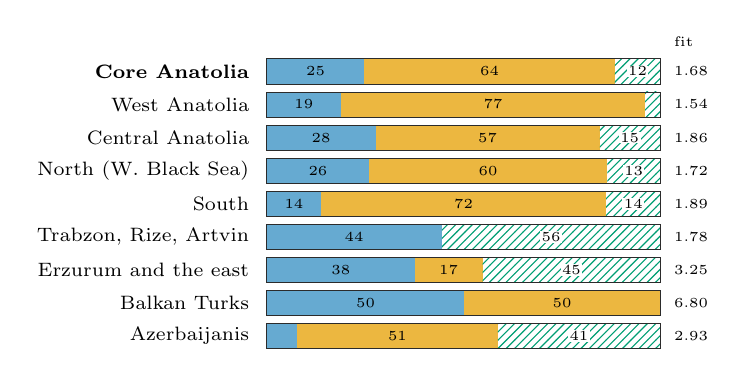
\begin{tikzpicture}[x=0.5mm, y=-4.2mm, font=\scriptsize]
  \node[anchor=east, font=\scriptsize\bfseries] at (-2,0) {Core Anatolia};
  \fill[tkblue!60] (0.0,0-0.38) rectangle (24.8,0+0.38);
  \node[font=\tiny] at (12.4,0) {25};
  \fill[tkorange!75] (24.8,0-0.38) rectangle (88.4,0+0.38);
  \node[font=\tiny] at (56.6,0) {64};
  \fill[tkgreen!55, pattern=north east lines, pattern color=tkgreen] (88.4,0-0.38) rectangle (100.0,0+0.38);
  \node[font=\tiny, fill=white, inner sep=0.5pt] at (94.2,0) {12};
  \draw[tkink, line width=0.3pt] (0,0-0.38) rectangle (100,0+0.38);
  \node[anchor=west, font=\tiny] at (101,0) {1.68};
  \node[anchor=east] at (-2,1) {West Anatolia};
  \fill[tkblue!60] (0.0,1-0.38) rectangle (18.9,1+0.38);
  \node[font=\tiny] at (9.4,1) {19};
  \fill[tkorange!75] (18.9,1-0.38) rectangle (96.1,1+0.38);
  \node[font=\tiny] at (57.5,1) {77};
  \fill[tkgreen!55, pattern=north east lines, pattern color=tkgreen] (96.1,1-0.38) rectangle (100.0,1+0.38);
  \draw[tkink, line width=0.3pt] (0,1-0.38) rectangle (100,1+0.38);
  \node[anchor=west, font=\tiny] at (101,1) {1.54};
  \node[anchor=east] at (-2,2) {Central Anatolia};
  \fill[tkblue!60] (0.0,2-0.38) rectangle (27.7,2+0.38);
  \node[font=\tiny] at (13.8,2) {28};
  \fill[tkorange!75] (27.7,2-0.38) rectangle (84.6,2+0.38);
  \node[font=\tiny] at (56.1,2) {57};
  \fill[tkgreen!55, pattern=north east lines, pattern color=tkgreen] (84.6,2-0.38) rectangle (99.9,2+0.38);
  \node[font=\tiny, fill=white, inner sep=0.5pt] at (92.2,2) {15};
  \draw[tkink, line width=0.3pt] (0,2-0.38) rectangle (100,2+0.38);
  \node[anchor=west, font=\tiny] at (101,2) {1.86};
  \node[anchor=east] at (-2,3) {North (W. Black Sea)};
  \fill[tkblue!60] (0.0,3-0.38) rectangle (26.0,3+0.38);
  \node[font=\tiny] at (13.0,3) {26};
  \fill[tkorange!75] (26.0,3-0.38) rectangle (86.5,3+0.38);
  \node[font=\tiny] at (56.2,3) {60};
  \fill[tkgreen!55, pattern=north east lines, pattern color=tkgreen] (86.5,3-0.38) rectangle (99.9,3+0.38);
  \node[font=\tiny, fill=white, inner sep=0.5pt] at (93.2,3) {13};
  \draw[tkink, line width=0.3pt] (0,3-0.38) rectangle (100,3+0.38);
  \node[anchor=west, font=\tiny] at (101,3) {1.72};
  \node[anchor=east] at (-2,4) {South};
  \fill[tkblue!60] (0.0,4-0.38) rectangle (13.8,4+0.38);
  \node[font=\tiny] at (6.9,4) {14};
  \fill[tkorange!75] (13.8,4-0.38) rectangle (86.2,4+0.38);
  \node[font=\tiny] at (50.0,4) {72};
  \fill[tkgreen!55, pattern=north east lines, pattern color=tkgreen] (86.2,4-0.38) rectangle (100.0,4+0.38);
  \node[font=\tiny, fill=white, inner sep=0.5pt] at (93.1,4) {14};
  \draw[tkink, line width=0.3pt] (0,4-0.38) rectangle (100,4+0.38);
  \node[anchor=west, font=\tiny] at (101,4) {1.89};
  \node[anchor=east] at (-2,5) {Trabzon, Rize, Artvin};
  \fill[tkblue!60] (0.0,5-0.38) rectangle (44.5,5+0.38);
  \node[font=\tiny] at (22.2,5) {44};
  \fill[tkgreen!55, pattern=north east lines, pattern color=tkgreen] (44.5,5-0.38) rectangle (100.0,5+0.38);
  \node[font=\tiny, fill=white, inner sep=0.5pt] at (72.2,5) {56};
  \draw[tkink, line width=0.3pt] (0,5-0.38) rectangle (100,5+0.38);
  \node[anchor=west, font=\tiny] at (101,5) {1.78};
  \node[anchor=east] at (-2,6) {Erzurum and the east};
  \fill[tkblue!60] (0.0,6-0.38) rectangle (37.6,6+0.38);
  \node[font=\tiny] at (18.8,6) {38};
  \fill[tkorange!75] (37.6,6-0.38) rectangle (54.8,6+0.38);
  \node[font=\tiny] at (46.2,6) {17};
  \fill[tkgreen!55, pattern=north east lines, pattern color=tkgreen] (54.8,6-0.38) rectangle (100.1,6+0.38);
  \node[font=\tiny, fill=white, inner sep=0.5pt] at (77.4,6) {45};
  \draw[tkink, line width=0.3pt] (0,6-0.38) rectangle (100,6+0.38);
  \node[anchor=west, font=\tiny] at (101,6) {3.25};
  \node[anchor=east] at (-2,7) {Balkan Turks};
  \fill[tkblue!60] (0.0,7-0.38) rectangle (50.1,7+0.38);
  \node[font=\tiny] at (25.1,7) {50};
  \fill[tkorange!75] (50.1,7-0.38) rectangle (100.0,7+0.38);
  \node[font=\tiny] at (75.0,7) {50};
  \draw[tkink, line width=0.3pt] (0,7-0.38) rectangle (100,7+0.38);
  \node[anchor=west, font=\tiny] at (101,7) {6.80};
  \node[anchor=east] at (-2,8) {Azerbaijanis};
  \fill[tkblue!60] (0.0,8-0.38) rectangle (7.8,8+0.38);
  \fill[tkorange!75] (7.8,8-0.38) rectangle (58.7,8+0.38);
  \node[font=\tiny] at (33.2,8) {51};
  \fill[tkgreen!55, pattern=north east lines, pattern color=tkgreen] (58.7,8-0.38) rectangle (100.0,8+0.38);
  \node[font=\tiny, fill=white, inner sep=0.5pt] at (79.3,8) {41};
  \draw[tkink, line width=0.3pt] (0,8-0.38) rectangle (100,8+0.38);
  \node[anchor=west, font=\tiny] at (101,8) {2.93};
  \node[anchor=west, font=\tiny] at (101,-0.9) {fit};
\end{tikzpicture}

\caption{Every region as Byzantine Anatolia (blue), Çapalıbağ as the early Anatolian Turkic source (orange) and Kartvelian (green, hatched), with the fit distance on the right.}
\label{fig:regions}
\end{figure}

\subsection{Subgroups}
Table~\ref{tab:subgroups} in the appendix fits the three models to every Turkish subgroup row with at least three people, plus the Yörük, Çepni and Manav rows. The most Turkic rows are in the west and south: Muğla and Bolu reach 37\% medieval Turkic, and the Yörük of Manisa, Mersin and Antalya 32\% to 36\%. Kayseri, Nevşehir, Kastamonu and Sivas sit lower, at about 17\%. The northeast (Trabzon, Rize, Gümüşhane, Bayburt, Artvin), the Meskhetian Turks and the Turkish Cypriots come out below 3\%. With these sources the model cannot separate their Caucasian or Levantine base from Turkic ancestry, so these low numbers do not measure it. Every Balkan row fits badly (fit above 4).

\subsection{The pre-Turkic layer}
Split into historical sources, the core average fits as 40.9\% Bronze Age Anatolia, 33.7\% Caucasus, 21.4\% medieval Turkic, 4.0\% Celtic and 0\% Greek (fit 1.60). Across six source sets the Turkic share stays between 19.6\% and 26.4\%. The Greek source gets 0\% in every set that includes Bronze Age Anatolia, and the Celtic share moves between 1\% and 14\%, too unstable to read. The pre-Turkic population was Anatolian, not Greek: it descends mostly from Bronze Age Anatolians and the Caucasus side. On the PCA (Fig.~\ref{fig:pca}), Byzantine and Bronze Age Anatolia sit apart from mainland Greeks.

\subsection{Where modern Anatolian Turks sit}
Fig.~\ref{fig:closeness} ranks populations by their distance from the core-Anatolian average. Azerbaijanis are closest (3.5 for the Caucasus average, 3.6 for Iran). The nearest Kurds are the western and Alevi Kurmanji of Malatya, Kayseri, Çorum and Kahramanmaraş (4.7), but they are closer still to Azerbaijanis (2.1) and to eastern Turks (2.2), so they belong to that eastern cluster. Kurds from the southeast, Iraq and Iran sit at 5.6. Anatolian and Pontic Greeks (7.0), North Caucasians and Armenians (7.2), mainland Greeks (8.3) and southern Italians (8.6) follow at similar distances. Turkmens, Oghuz but far more East Eurasian, sit at 9.9. Uzbeks are at 20.5, Kazakhs at 32.2 and Kyrgyz at 35.7.

\begin{figure}[t]
\centering
% Generated by analysis/10_paper_figures.py from results/closeness.json.
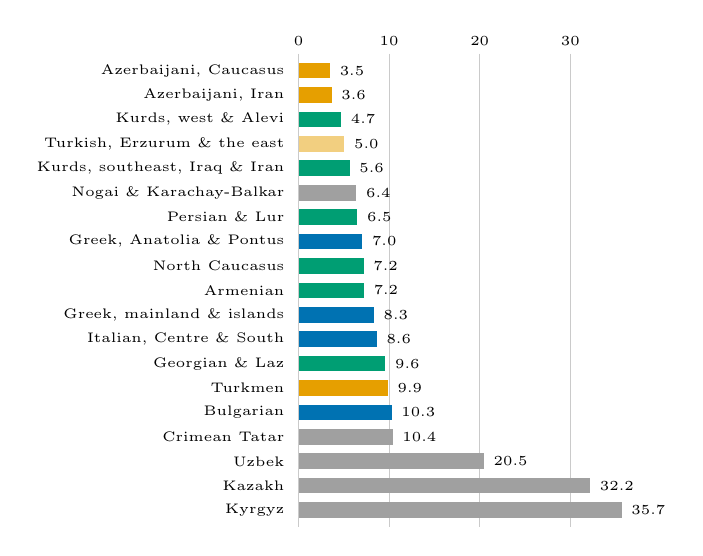
\begin{tikzpicture}[x=1.15mm, y=-3.1mm, font=\scriptsize]
  \draw[tkink!25] (0,-0.7) -- (0,18.7); \node[font=\tiny] at (0,-1.2) {0};
  \draw[tkink!25] (10,-0.7) -- (10,18.7); \node[font=\tiny] at (10,-1.2) {10};
  \draw[tkink!25] (20,-0.7) -- (20,18.7); \node[font=\tiny] at (20,-1.2) {20};
  \draw[tkink!25] (30,-0.7) -- (30,18.7); \node[font=\tiny] at (30,-1.2) {30};
  \node[anchor=east, font=\tiny] at (-0.5,0) {Azerbaijani, Caucasus};
  \fill[tkorange] (0,0-0.32) rectangle (3.47,0+0.32);
  \node[anchor=west, font=\tiny] at (3.47,0) {3.5};
  \node[anchor=east, font=\tiny] at (-0.5,1) {Azerbaijani, Iran};
  \fill[tkorange] (0,1-0.32) rectangle (3.64,1+0.32);
  \node[anchor=west, font=\tiny] at (3.64,1) {3.6};
  \node[anchor=east, font=\tiny] at (-0.5,2) {Kurds, west \& Alevi};
  \fill[tkgreen] (0,2-0.32) rectangle (4.69,2+0.32);
  \node[anchor=west, font=\tiny] at (4.69,2) {4.7};
  \node[anchor=east, font=\tiny] at (-0.5,3) {Turkish, Erzurum \& the east};
  \fill[tkorange!50] (0,3-0.32) rectangle (5.05,3+0.32);
  \node[anchor=west, font=\tiny] at (5.05,3) {5.0};
  \node[anchor=east, font=\tiny] at (-0.5,4) {Kurds, southeast, Iraq \& Iran};
  \fill[tkgreen] (0,4-0.32) rectangle (5.64,4+0.32);
  \node[anchor=west, font=\tiny] at (5.64,4) {5.6};
  \node[anchor=east, font=\tiny] at (-0.5,5) {Nogai \& Karachay-Balkar};
  \fill[tkink!45] (0,5-0.32) rectangle (6.38,5+0.32);
  \node[anchor=west, font=\tiny] at (6.38,5) {6.4};
  \node[anchor=east, font=\tiny] at (-0.5,6) {Persian \& Lur};
  \fill[tkgreen] (0,6-0.32) rectangle (6.50,6+0.32);
  \node[anchor=west, font=\tiny] at (6.50,6) {6.5};
  \node[anchor=east, font=\tiny] at (-0.5,7) {Greek, Anatolia \& Pontus};
  \fill[tkblue] (0,7-0.32) rectangle (7.03,7+0.32);
  \node[anchor=west, font=\tiny] at (7.03,7) {7.0};
  \node[anchor=east, font=\tiny] at (-0.5,8) {North Caucasus};
  \fill[tkgreen] (0,8-0.32) rectangle (7.18,8+0.32);
  \node[anchor=west, font=\tiny] at (7.18,8) {7.2};
  \node[anchor=east, font=\tiny] at (-0.5,9) {Armenian};
  \fill[tkgreen] (0,9-0.32) rectangle (7.22,9+0.32);
  \node[anchor=west, font=\tiny] at (7.22,9) {7.2};
  \node[anchor=east, font=\tiny] at (-0.5,10) {Greek, mainland \& islands};
  \fill[tkblue] (0,10-0.32) rectangle (8.32,10+0.32);
  \node[anchor=west, font=\tiny] at (8.32,10) {8.3};
  \node[anchor=east, font=\tiny] at (-0.5,11) {Italian, Centre \& South};
  \fill[tkblue] (0,11-0.32) rectangle (8.63,11+0.32);
  \node[anchor=west, font=\tiny] at (8.63,11) {8.6};
  \node[anchor=east, font=\tiny] at (-0.5,12) {Georgian \& Laz};
  \fill[tkgreen] (0,12-0.32) rectangle (9.59,12+0.32);
  \node[anchor=west, font=\tiny] at (9.59,12) {9.6};
  \node[anchor=east, font=\tiny] at (-0.5,13) {Turkmen};
  \fill[tkorange] (0,13-0.32) rectangle (9.86,13+0.32);
  \node[anchor=west, font=\tiny] at (9.86,13) {9.9};
  \node[anchor=east, font=\tiny] at (-0.5,14) {Bulgarian};
  \fill[tkblue] (0,14-0.32) rectangle (10.27,14+0.32);
  \node[anchor=west, font=\tiny] at (10.27,14) {10.3};
  \node[anchor=east, font=\tiny] at (-0.5,15) {Crimean Tatar};
  \fill[tkink!45] (0,15-0.32) rectangle (10.39,15+0.32);
  \node[anchor=west, font=\tiny] at (10.39,15) {10.4};
  \node[anchor=east, font=\tiny] at (-0.5,16) {Uzbek};
  \fill[tkink!45] (0,16-0.32) rectangle (20.47,16+0.32);
  \node[anchor=west, font=\tiny] at (20.47,16) {20.5};
  \node[anchor=east, font=\tiny] at (-0.5,17) {Kazakh};
  \fill[tkink!45] (0,17-0.32) rectangle (32.20,17+0.32);
  \node[anchor=west, font=\tiny] at (32.20,17) {32.2};
  \node[anchor=east, font=\tiny] at (-0.5,18) {Kyrgyz};
  \fill[tkink!45] (0,18-0.32) rectangle (35.68,18+0.32);
  \node[anchor=west, font=\tiny] at (35.68,18) {35.7};
\end{tikzpicture}

\caption{G25 distance ($\times 100$) from the core-Anatolian Turkish average. Orange: Oghuz Turkic and Turkish; green: West Asia and the Caucasus; blue: Europe; grey: other Turkic peoples.}
\label{fig:closeness}
\end{figure}

\begin{figure*}[t]
\centering
\resizebox{\textwidth}{!}{% Generated by analysis/10_paper_figures.py from the PCA output (07_pca.py).
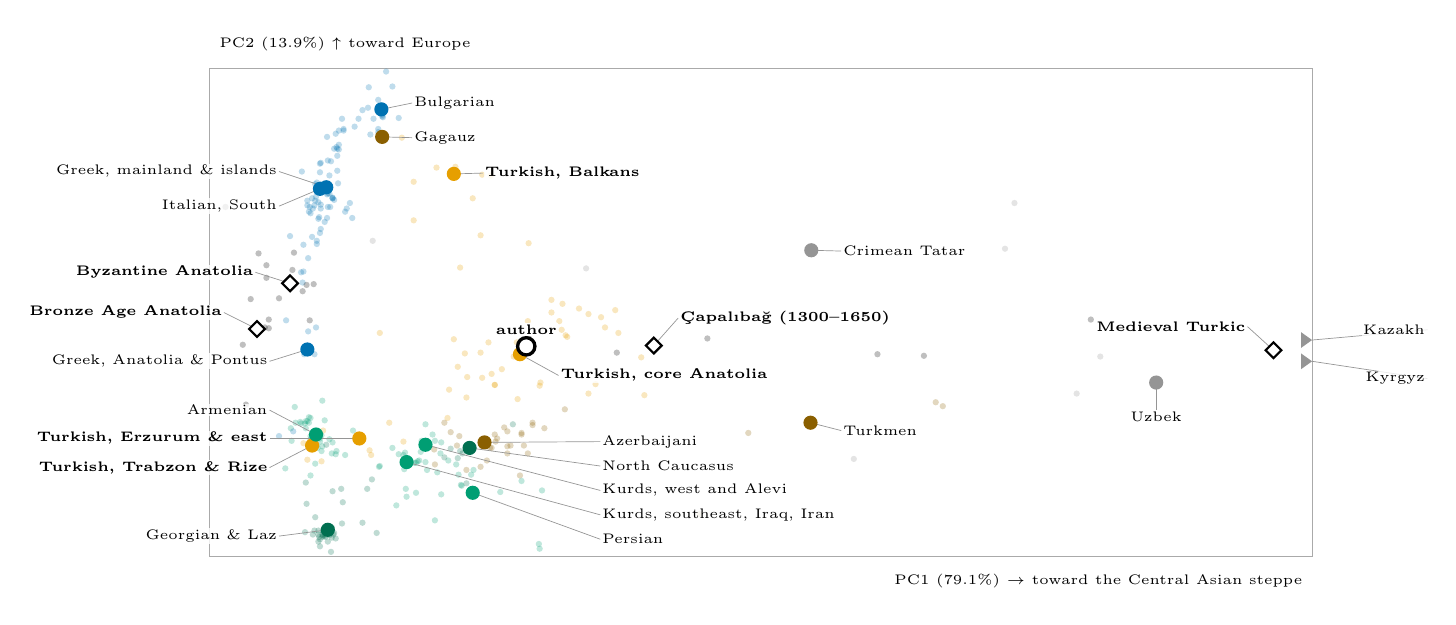
\begin{tikzpicture}[x=1mm, y=1mm, font=\tiny]
  \draw[tkink!40] (0,0) rectangle (140,62);
  \node[anchor=north east] at (140,-1) {PC1 (79.1\%) $\rightarrow$ toward the Central Asian steppe};
  \node[anchor=south west] at (0,63) {PC2 (13.9\%) $\uparrow$ toward Europe};
  \fill[tkorange, opacity=0.25] (40.8,29.1) circle (0.4);
  \fill[tkorange, opacity=0.25] (37.1,23.8) circle (0.4);
  \fill[tkorange, opacity=0.25] (49.7,30.4) circle (0.4);
  \fill[tkorange, opacity=0.25] (39.1,20.0) circle (0.4);
  \fill[tkorange, opacity=0.25] (51.9,28.4) circle (0.4);
  \fill[tkorange, opacity=0.25] (48.1,30.8) circle (0.4);
  \fill[tkorange, opacity=0.25] (40.5,39.8) circle (0.4);
  \fill[tkorange, opacity=0.25] (55.2,20.5) circle (0.4);
  \fill[tkorange, opacity=0.25] (39.0,27.2) circle (0.4);
  \fill[tkorange, opacity=0.25] (45.4,27.9) circle (0.4);
  \fill[tkorange, opacity=0.25] (44.8,32.1) circle (0.4);
  \fill[tkorange, opacity=0.25] (46.9,31.5) circle (0.4);
  \fill[tkorange, opacity=0.25] (35.4,27.2) circle (0.4);
  \fill[tkorange, opacity=0.25] (34.6,22.7) circle (0.4);
  \fill[tkorange, opacity=0.25] (50.2,29.1) circle (0.4);
  \fill[tkorange, opacity=0.25] (44.7,28.8) circle (0.4);
  \fill[tkorange, opacity=0.25] (44.4,29.9) circle (0.4);
  \fill[tkorange, opacity=0.25] (48.1,20.7) circle (0.4);
  \fill[tkorange, opacity=0.25] (40.4,29.9) circle (0.4);
  \fill[tkorange, opacity=0.25] (31.0,27.6) circle (0.4);
  \fill[tkorange, opacity=0.25] (32.7,22.8) circle (0.4);
  \fill[tkorange, opacity=0.25] (42.0,22.1) circle (0.4);
  \fill[tkorange, opacity=0.25] (41.9,21.7) circle (0.4);
  \fill[tkorange, opacity=0.25] (43.4,32.6) circle (0.4);
  \fill[tkorange, opacity=0.25] (38.6,25.4) circle (0.4);
  \fill[tkorange, opacity=0.25] (43.4,31.0) circle (0.4);
  \fill[tkorange, opacity=0.25] (49.0,21.9) circle (0.4);
  \fill[tkorange, opacity=0.25] (54.8,25.3) circle (0.4);
  \fill[tkorange, opacity=0.25] (31.5,24.1) circle (0.4);
  \fill[tkorange, opacity=0.25] (32.4,25.8) circle (0.4);
  \fill[tkorange, opacity=0.25] (51.5,31.3) circle (0.4);
  \fill[tkorange, opacity=0.25] (35.8,23.2) circle (0.4);
  \fill[tkorange, opacity=0.25] (34.4,25.9) circle (0.4);
  \fill[tkorange, opacity=0.25] (21.6,28.4) circle (0.4);
  \fill[tkorange, opacity=0.25] (32.6,20.2) circle (0.4);
  \fill[tkorange, opacity=0.25] (36.2,21.8) circle (0.4);
  \fill[tkorange, opacity=0.25] (43.8,28.6) circle (0.4);
  \fill[tkorange, opacity=0.25] (31.8,36.7) circle (0.4);
  \fill[tkorange, opacity=0.25] (36.2,21.8) circle (0.4);
  \fill[tkorange, opacity=0.25] (45.2,28.1) circle (0.4);
  \fill[tkorange, opacity=0.25] (14.2,12.1) circle (0.4);
  \fill[tkorange, opacity=0.25] (12.4,12.3) circle (0.4);
  \fill[tkorange, opacity=0.25] (11.9,14.4) circle (0.4);
  \fill[tkorange, opacity=0.25] (30.4,21.2) circle (0.4);
  \fill[tkorange, opacity=0.25] (30.2,17.6) circle (0.4);
  \fill[tkorange, opacity=0.25] (14.4,16.0) circle (0.4);
  \fill[tkorange, opacity=0.25] (22.8,17.0) circle (0.4);
  \fill[tkorange, opacity=0.25] (20.5,12.9) circle (0.4);
  \fill[tkorange, opacity=0.25] (20.3,13.5) circle (0.4);
  \fill[tkorange, opacity=0.25] (13.6,14.2) circle (0.4);
  \fill[tkorange, opacity=0.25] (24.6,14.6) circle (0.4);
  \fill[tkorange, opacity=0.25] (33.4,45.5) circle (0.4);
  \fill[tkorange, opacity=0.25] (25.9,47.6) circle (0.4);
  \fill[tkorange, opacity=0.25] (31.2,49.5) circle (0.4);
  \fill[tkorange, opacity=0.25] (34.4,40.8) circle (0.4);
  \fill[tkorange, opacity=0.25] (34.6,48.5) circle (0.4);
  \fill[tkorange, opacity=0.25] (25.9,42.7) circle (0.4);
  \fill[tkorange, opacity=0.25] (28.8,49.4) circle (0.4);
  \fill[tkorange, opacity=0.25] (24.4,53.2) circle (0.4);
  \fill[tkorange, opacity=0.25] (35.7,48.4) circle (0.4);
  \fill[tkorange!60!black, opacity=0.25] (31.7,15.3) circle (0.4);
  \fill[tkorange!60!black, opacity=0.25] (35.2,14.5) circle (0.4);
  \fill[tkorange!60!black, opacity=0.25] (34.6,14.0) circle (0.4);
  \fill[tkorange!60!black, opacity=0.25] (41.0,17.0) circle (0.4);
  \fill[tkorange!60!black, opacity=0.25] (38.2,14.1) circle (0.4);
  \fill[tkorange!60!black, opacity=0.25] (37.8,15.9) circle (0.4);
  \fill[tkorange!60!black, opacity=0.25] (42.5,16.3) circle (0.4);
  \fill[tkorange!60!black, opacity=0.25] (31.4,14.1) circle (0.4);
  \fill[tkorange!60!black, opacity=0.25] (34.4,11.4) circle (0.4);
  \fill[tkorange!60!black, opacity=0.25] (30.6,15.8) circle (0.4);
  \fill[tkorange!60!black, opacity=0.25] (28.5,13.6) circle (0.4);
  \fill[tkorange!60!black, opacity=0.25] (36.5,15.0) circle (0.4);
  \fill[tkorange!60!black, opacity=0.25] (39.6,15.7) circle (0.4);
  \fill[tkorange!60!black, opacity=0.25] (33.2,14.0) circle (0.4);
  \fill[tkorange!60!black, opacity=0.25] (27.4,14.6) circle (0.4);
  \fill[tkorange!60!black, opacity=0.25] (45.1,18.7) circle (0.4);
  \fill[tkorange!60!black, opacity=0.25] (32.6,11.0) circle (0.4);
  \fill[tkorange!60!black, opacity=0.25] (33.1,14.1) circle (0.4);
  \fill[tkorange!60!black, opacity=0.25] (39.6,15.5) circle (0.4);
  \fill[tkorange!60!black, opacity=0.25] (35.6,13.8) circle (0.4);
  \fill[tkorange!60!black, opacity=0.25] (35.8,13.8) circle (0.4);
  \fill[tkorange!60!black, opacity=0.25] (41.0,16.7) circle (0.4);
  \fill[tkorange!60!black, opacity=0.25] (29.8,17.0) circle (0.4);
  \fill[tkorange!60!black, opacity=0.25] (40.4,13.1) circle (0.4);
  \fill[tkorange!60!black, opacity=0.25] (37.8,13.1) circle (0.4);
  \fill[tkorange!60!black, opacity=0.25] (39.4,10.3) circle (0.4);
  \fill[tkorange!60!black, opacity=0.25] (37.8,14.0) circle (0.4);
  \fill[tkorange!60!black, opacity=0.25] (36.3,14.6) circle (0.4);
  \fill[tkorange!60!black, opacity=0.25] (39.9,14.1) circle (0.4);
  \fill[tkorange!60!black, opacity=0.25] (35.2,12.2) circle (0.4);
  \fill[tkorange!60!black, opacity=0.25] (36.2,15.5) circle (0.4);
  \fill[tkorange!60!black, opacity=0.25] (37.4,16.4) circle (0.4);
  \fill[tkorange!60!black, opacity=0.25] (92.2,19.6) circle (0.4);
  \fill[tkorange!60!black, opacity=0.25] (62.2,5.4) circle (0.4);
  \fill[tkorange!60!black, opacity=0.25] (68.4,15.7) circle (0.4);
  \fill[tkorange!60!black, opacity=0.25] (28.6,11.7) circle (0.4);
  \fill[tkorange!60!black, opacity=0.25] (93.1,19.1) circle (0.4);
  \fill[tkorange!60!black, opacity=0.25] (21.9,53.3) circle (0.4);
  \fill[tkink!50, opacity=0.25] (120.2,21.7) circle (0.4);
  \fill[tkink!50, opacity=0.25] (81.8,12.4) circle (0.4);
  \fill[tkink!50, opacity=0.25] (113.1,25.4) circle (0.4);
  \fill[tkink!50, opacity=0.25] (110.1,20.7) circle (0.4);
  \fill[tkink!50, opacity=0.25] (20.7,40.1) circle (0.4);
  \fill[tkink!50, opacity=0.25] (47.8,36.6) circle (0.4);
  \fill[tkink!50, opacity=0.25] (101.0,39.1) circle (0.4);
  \fill[tkink!50, opacity=0.25] (102.2,44.9) circle (0.4);
  \fill[tkgreen, opacity=0.25] (29.4,14.5) circle (0.4);
  \fill[tkgreen, opacity=0.25] (27.4,16.8) circle (0.4);
  \fill[tkgreen, opacity=0.25] (26.9,14.7) circle (0.4);
  \fill[tkgreen, opacity=0.25] (28.3,15.5) circle (0.4);
  \fill[tkgreen, opacity=0.25] (26.8,13.3) circle (0.4);
  \fill[tkgreen, opacity=0.25] (28.6,14.7) circle (0.4);
  \fill[tkgreen, opacity=0.25] (24.8,13.2) circle (0.4);
  \fill[tkgreen, opacity=0.25] (33.5,11.0) circle (0.4);
  \fill[tkgreen, opacity=0.25] (26.6,12.2) circle (0.4);
  \fill[tkgreen, opacity=0.25] (25.0,12.3) circle (0.4);
  \fill[tkgreen, opacity=0.25] (24.6,12.2) circle (0.4);
  \fill[tkgreen, opacity=0.25] (21.6,11.5) circle (0.4);
  \fill[tkgreen, opacity=0.25] (23.2,13.8) circle (0.4);
  \fill[tkgreen, opacity=0.25] (24.0,13.0) circle (0.4);
  \fill[tkgreen, opacity=0.25] (24.7,11.1) circle (0.4);
  \fill[tkgreen, opacity=0.25] (24.9,8.6) circle (0.4);
  \fill[tkgreen, opacity=0.25] (25.0,7.6) circle (0.4);
  \fill[tkgreen, opacity=0.25] (28.9,10.7) circle (0.4);
  \fill[tkgreen, opacity=0.25] (26.4,12.1) circle (0.4);
  \fill[tkgreen, opacity=0.25] (24.6,12.9) circle (0.4);
  \fill[tkgreen, opacity=0.25] (29.3,13.1) circle (0.4);
  \fill[tkgreen, opacity=0.25] (26.0,11.9) circle (0.4);
  \fill[tkgreen, opacity=0.25] (21.5,11.4) circle (0.4);
  \fill[tkgreen, opacity=0.25] (13.6,15.5) circle (0.4);
  \fill[tkgreen, opacity=0.25] (10.3,16.3) circle (0.4);
  \fill[tkgreen, opacity=0.25] (11.5,17.1) circle (0.4);
  \fill[tkgreen, opacity=0.25] (12.4,17.2) circle (0.4);
  \fill[tkgreen, opacity=0.25] (13.0,15.3) circle (0.4);
  \fill[tkgreen, opacity=0.25] (13.8,15.3) circle (0.4);
  \fill[tkgreen, opacity=0.25] (15.6,14.5) circle (0.4);
  \fill[tkgreen, opacity=0.25] (16.0,13.0) circle (0.4);
  \fill[tkgreen, opacity=0.25] (9.6,11.2) circle (0.4);
  \fill[tkgreen, opacity=0.25] (14.0,14.6) circle (0.4);
  \fill[tkgreen, opacity=0.25] (12.2,17.2) circle (0.4);
  \fill[tkgreen, opacity=0.25] (14.2,13.4) circle (0.4);
  \fill[tkgreen, opacity=0.25] (16.1,13.4) circle (0.4);
  \fill[tkgreen, opacity=0.25] (17.2,12.9) circle (0.4);
  \fill[tkgreen, opacity=0.25] (14.6,17.3) circle (0.4);
  \fill[tkgreen, opacity=0.25] (12.8,15.3) circle (0.4);
  \fill[tkgreen, opacity=0.25] (10.9,17.0) circle (0.4);
  \fill[tkgreen, opacity=0.25] (10.8,19.0) circle (0.4);
  \fill[tkgreen, opacity=0.25] (12.8,10.3) circle (0.4);
  \fill[tkgreen, opacity=0.25] (14.3,14.0) circle (0.4);
  \fill[tkgreen, opacity=0.25] (14.3,19.8) circle (0.4);
  \fill[tkgreen, opacity=0.25] (13.4,11.8) circle (0.4);
  \fill[tkgreen, opacity=0.25] (12.8,17.6) circle (0.4);
  \fill[tkgreen, opacity=0.25] (12.1,16.9) circle (0.4);
  \fill[tkgreen, opacity=0.25] (12.6,17.0) circle (0.4);
  \fill[tkgreen, opacity=0.25] (15.5,13.1) circle (0.4);
  \fill[tkgreen, opacity=0.25] (11.6,16.9) circle (0.4);
  \fill[tkgreen, opacity=0.25] (12.8,14.9) circle (0.4);
  \fill[tkgreen, opacity=0.25] (13.2,15.4) circle (0.4);
  \fill[tkgreen, opacity=0.25] (13.6,15.8) circle (0.4);
  \fill[tkgreen, opacity=0.25] (10.4,14.7) circle (0.4);
  \fill[tkgreen, opacity=0.25] (12.6,17.7) circle (0.4);
  \fill[tkgreen, opacity=0.25] (18.2,16.0) circle (0.4);
  \fill[tkgreen, opacity=0.25] (15.2,14.9) circle (0.4);
  \fill[tkgreen, opacity=0.25] (14.2,15.4) circle (0.4);
  \fill[tkgreen, opacity=0.25] (12.2,16.3) circle (0.4);
  \fill[tkgreen, opacity=0.25] (13.7,13.8) circle (0.4);
  \fill[tkgreen, opacity=0.25] (14.0,15.0) circle (0.4);
  \fill[tkgreen, opacity=0.25] (26.2,8.1) circle (0.4);
  \fill[tkgreen, opacity=0.25] (27.6,11.0) circle (0.4);
  \fill[tkgreen, opacity=0.25] (41.9,1.0) circle (0.4);
  \fill[tkgreen, opacity=0.25] (28.6,4.6) circle (0.4);
  \fill[tkgreen, opacity=0.25] (29.4,7.9) circle (0.4);
  \fill[tkgreen, opacity=0.25] (33.3,8.3) circle (0.4);
  \fill[tkgreen, opacity=0.25] (23.7,6.5) circle (0.4);
  \fill[tkgreen, opacity=0.25] (31.9,9.1) circle (0.4);
  \fill[tkgreen, opacity=0.25] (31.3,11.7) circle (0.4);
  \fill[tkgreen, opacity=0.25] (33.2,10.4) circle (0.4);
  \fill[tkgreen, opacity=0.25] (36.9,8.2) circle (0.4);
  \fill[tkgreen, opacity=0.25] (42.2,8.4) circle (0.4);
  \fill[tkgreen, opacity=0.25] (26.2,11.9) circle (0.4);
  \fill[tkgreen, opacity=0.25] (31.6,10.4) circle (0.4);
  \fill[tkgreen, opacity=0.25] (30.3,12.2) circle (0.4);
  \fill[tkgreen, opacity=0.25] (39.6,9.6) circle (0.4);
  \fill[tkgreen, opacity=0.25] (41.8,1.6) circle (0.4);
  \fill[tkgreen, opacity=0.25] (27.4,12.0) circle (0.4);
  \fill[tkgreen, opacity=0.25] (32.0,9.0) circle (0.4);
  \fill[tkgreen!70!black, opacity=0.25] (13.4,5.0) circle (0.4);
  \fill[tkgreen!70!black, opacity=0.25] (12.1,3.1) circle (0.4);
  \fill[tkgreen!70!black, opacity=0.25] (13.8,3.3) circle (0.4);
  \fill[tkgreen!70!black, opacity=0.25] (12.3,6.7) circle (0.4);
  \fill[tkgreen!70!black, opacity=0.25] (15.6,8.3) circle (0.4);
  \fill[tkgreen!70!black, opacity=0.25] (16.7,8.6) circle (0.4);
  \fill[tkgreen!70!black, opacity=0.25] (20.6,9.8) circle (0.4);
  \fill[tkgreen!70!black, opacity=0.25] (19.4,4.3) circle (0.4);
  \fill[tkgreen!70!black, opacity=0.25] (14.8,14.2) circle (0.4);
  \fill[tkgreen!70!black, opacity=0.25] (16.9,6.9) circle (0.4);
  \fill[tkgreen!70!black, opacity=0.25] (20.0,8.6) circle (0.4);
  \fill[tkgreen!70!black, opacity=0.25] (15.4,0.6) circle (0.4);
  \fill[tkgreen!70!black, opacity=0.25] (15.4,3.3) circle (0.4);
  \fill[tkgreen!70!black, opacity=0.25] (13.3,3.3) circle (0.4);
  \fill[tkgreen!70!black, opacity=0.25] (12.2,9.4) circle (0.4);
  \fill[tkgreen!70!black, opacity=0.25] (14.4,2.7) circle (0.4);
  \fill[tkgreen!70!black, opacity=0.25] (15.0,1.9) circle (0.4);
  \fill[tkgreen!70!black, opacity=0.25] (13.1,2.8) circle (0.4);
  \fill[tkgreen!70!black, opacity=0.25] (15.2,2.7) circle (0.4);
  \fill[tkgreen!70!black, opacity=0.25] (14.6,2.6) circle (0.4);
  \fill[tkgreen!70!black, opacity=0.25] (13.8,1.9) circle (0.4);
  \fill[tkgreen!70!black, opacity=0.25] (15.5,2.4) circle (0.4);
  \fill[tkgreen!70!black, opacity=0.25] (14.0,1.3) circle (0.4);
  \fill[tkgreen!70!black, opacity=0.25] (14.7,2.5) circle (0.4);
  \fill[tkgreen!70!black, opacity=0.25] (15.3,3.0) circle (0.4);
  \fill[tkgreen!70!black, opacity=0.25] (14.3,2.5) circle (0.4);
  \fill[tkgreen!70!black, opacity=0.25] (13.8,2.8) circle (0.4);
  \fill[tkgreen!70!black, opacity=0.25] (14.4,3.2) circle (0.4);
  \fill[tkgreen!70!black, opacity=0.25] (14.5,3.2) circle (0.4);
  \fill[tkgreen!70!black, opacity=0.25] (15.5,3.7) circle (0.4);
  \fill[tkgreen!70!black, opacity=0.25] (14.3,2.8) circle (0.4);
  \fill[tkgreen!70!black, opacity=0.25] (14.8,3.1) circle (0.4);
  \fill[tkgreen!70!black, opacity=0.25] (14.0,2.2) circle (0.4);
  \fill[tkgreen!70!black, opacity=0.25] (14.6,2.8) circle (0.4);
  \fill[tkgreen!70!black, opacity=0.25] (16.8,4.2) circle (0.4);
  \fill[tkgreen!70!black, opacity=0.25] (13.9,2.5) circle (0.4);
  \fill[tkgreen!70!black, opacity=0.25] (15.7,2.8) circle (0.4);
  \fill[tkgreen!70!black, opacity=0.25] (16.0,2.3) circle (0.4);
  \fill[tkgreen!70!black, opacity=0.25] (15.8,3.0) circle (0.4);
  \fill[tkgreen!70!black, opacity=0.25] (21.2,3.0) circle (0.4);
  \fill[tkgreen!70!black, opacity=0.25] (31.8,13.4) circle (0.4);
  \fill[tkgreen!70!black, opacity=0.25] (29.8,12.6) circle (0.4);
  \fill[tkgreen!70!black, opacity=0.25] (30.6,13.7) circle (0.4);
  \fill[tkgreen!70!black, opacity=0.25] (38.5,16.8) circle (0.4);
  \fill[tkgreen!70!black, opacity=0.25] (32.1,13.1) circle (0.4);
  \fill[tkgreen!70!black, opacity=0.25] (31.5,12.5) circle (0.4);
  \fill[tkgreen!70!black, opacity=0.25] (32.7,13.6) circle (0.4);
  \fill[tkgreen!70!black, opacity=0.25] (32.6,9.3) circle (0.4);
  \fill[tkblue, opacity=0.25] (16.4,52.3) circle (0.4);
  \fill[tkblue, opacity=0.25] (13.6,47.5) circle (0.4);
  \fill[tkblue, opacity=0.25] (16.4,54.1) circle (0.4);
  \fill[tkblue, opacity=0.25] (14.9,53.3) circle (0.4);
  \fill[tkblue, opacity=0.25] (17.0,54.1) circle (0.4);
  \fill[tkblue, opacity=0.25] (13.0,40.6) circle (0.4);
  \fill[tkblue, opacity=0.25] (14.9,43.0) circle (0.4);
  \fill[tkblue, opacity=0.25] (14.0,41.1) circle (0.4);
  \fill[tkblue, opacity=0.25] (14.1,41.6) circle (0.4);
  \fill[tkblue, opacity=0.25] (14.6,42.5) circle (0.4);
  \fill[tkblue, opacity=0.25] (10.2,40.7) circle (0.4);
  \fill[tkblue, opacity=0.25] (15.6,45.5) circle (0.4);
  \fill[tkblue, opacity=0.25] (13.8,45.0) circle (0.4);
  \fill[tkblue, opacity=0.25] (17.2,43.8) circle (0.4);
  \fill[tkblue, opacity=0.25] (15.0,44.4) circle (0.4);
  \fill[tkblue, opacity=0.25] (13.6,40.1) circle (0.4);
  \fill[tkblue, opacity=0.25] (17.4,44.2) circle (0.4);
  \fill[tkblue, opacity=0.25] (13.9,43.1) circle (0.4);
  \fill[tkblue, opacity=0.25] (11.9,39.6) circle (0.4);
  \fill[tkblue, opacity=0.25] (13.8,42.9) circle (0.4);
  \fill[tkblue, opacity=0.25] (11.8,34.8) circle (0.4);
  \fill[tkblue, opacity=0.25] (12.5,37.9) circle (0.4);
  \fill[tkblue, opacity=0.25] (13.6,39.7) circle (0.4);
  \fill[tkblue, opacity=0.25] (16.3,47.4) circle (0.4);
  \fill[tkblue, opacity=0.25] (11.9,36.2) circle (0.4);
  \fill[tkblue, opacity=0.25] (11.6,36.1) circle (0.4);
  \fill[tkblue, opacity=0.25] (16.0,53.7) circle (0.4);
  \fill[tkblue, opacity=0.25] (18.4,54.6) circle (0.4);
  \fill[tkblue, opacity=0.25] (16.1,52.0) circle (0.4);
  \fill[tkblue, opacity=0.25] (16.2,51.8) circle (0.4);
  \fill[tkblue, opacity=0.25] (16.2,50.9) circle (0.4);
  \fill[tkblue, opacity=0.25] (15.0,50.3) circle (0.4);
  \fill[tkblue, opacity=0.25] (14.0,49.9) circle (0.4);
  \fill[tkblue, opacity=0.25] (12.7,44.4) circle (0.4);
  \fill[tkblue, opacity=0.25] (14.0,48.8) circle (0.4);
  \fill[tkblue, opacity=0.25] (16.8,55.6) circle (0.4);
  \fill[tkblue, opacity=0.25] (16.4,51.7) circle (0.4);
  \fill[tkblue, opacity=0.25] (15.4,50.2) circle (0.4);
  \fill[tkblue, opacity=0.25] (15.8,51.8) circle (0.4);
  \fill[tkblue, opacity=0.25] (17.0,54.3) circle (0.4);
  \fill[tkblue, opacity=0.25] (12.9,14.0) circle (0.4);
  \fill[tkblue, opacity=0.25] (8.8,15.3) circle (0.4);
  \fill[tkblue, opacity=0.25] (13.3,25.7) circle (0.4);
  \fill[tkblue, opacity=0.25] (12.0,25.7) circle (0.4);
  \fill[tkblue, opacity=0.25] (9.7,30.0) circle (0.4);
  \fill[tkblue, opacity=0.25] (12.5,28.6) circle (0.4);
  \fill[tkblue, opacity=0.25] (13.5,29.1) circle (0.4);
  \fill[tkblue, opacity=0.25] (13.4,47.3) circle (0.4);
  \fill[tkblue, opacity=0.25] (10.6,15.9) circle (0.4);
  \fill[tkblue, opacity=0.25] (15.2,46.1) circle (0.4);
  \fill[tkblue, opacity=0.25] (14.1,50.0) circle (0.4);
  \fill[tkblue, opacity=0.25] (15.3,44.4) circle (0.4);
  \fill[tkblue, opacity=0.25] (15.6,45.5) circle (0.4);
  \fill[tkblue, opacity=0.25] (18.1,43.0) circle (0.4);
  \fill[tkblue, opacity=0.25] (13.3,44.6) circle (0.4);
  \fill[tkblue, opacity=0.25] (17.8,44.9) circle (0.4);
  \fill[tkblue, opacity=0.25] (14.9,46.0) circle (0.4);
  \fill[tkblue, opacity=0.25] (15.8,45.3) circle (0.4);
  \fill[tkblue, opacity=0.25] (22.1,56.5) circle (0.4);
  \fill[tkblue, opacity=0.25] (20.2,59.6) circle (0.4);
  \fill[tkblue, opacity=0.25] (21.9,56.1) circle (0.4);
  \fill[tkblue, opacity=0.25] (18.9,55.6) circle (0.4);
  \fill[tkblue, opacity=0.25] (21.4,58.0) circle (0.4);
  \fill[tkblue, opacity=0.25] (19.4,56.7) circle (0.4);
  \fill[tkblue, opacity=0.25] (23.2,59.7) circle (0.4);
  \fill[tkblue, opacity=0.25] (20.1,57.0) circle (0.4);
  \fill[tkblue, opacity=0.25] (24.0,55.7) circle (0.4);
  \fill[tkblue, opacity=0.25] (21.4,54.3) circle (0.4);
  \fill[tkblue, opacity=0.25] (21.9,55.9) circle (0.4);
  \fill[tkblue, opacity=0.25] (21.4,53.9) circle (0.4);
  \fill[tkblue, opacity=0.25] (20.8,55.6) circle (0.4);
  \fill[tkblue, opacity=0.25] (22.0,55.8) circle (0.4);
  \fill[tkblue, opacity=0.25] (22.4,61.6) circle (0.4);
  \fill[tkblue, opacity=0.25] (20.4,53.6) circle (0.4);
  \fill[tkblue, opacity=0.25] (14.1,47.3) circle (0.4);
  \fill[tkblue, opacity=0.25] (14.1,44.7) circle (0.4);
  \fill[tkblue, opacity=0.25] (14.1,46.5) circle (0.4);
  \fill[tkblue, opacity=0.25] (12.6,43.8) circle (0.4);
  \fill[tkblue, opacity=0.25] (13.1,44.2) circle (0.4);
  \fill[tkblue, opacity=0.25] (12.8,43.6) circle (0.4);
  \fill[tkblue, opacity=0.25] (13.5,45.7) circle (0.4);
  \fill[tkblue, opacity=0.25] (11.7,48.9) circle (0.4);
  \fill[tkblue, opacity=0.25] (13.4,45.2) circle (0.4);
  \fill[tkblue, opacity=0.25] (13.0,45.5) circle (0.4);
  \fill[tkblue, opacity=0.25] (15.6,45.6) circle (0.4);
  \fill[tkblue, opacity=0.25] (12.4,45.2) circle (0.4);
  \fill[tkblue, opacity=0.25] (13.8,46.8) circle (0.4);
  \fill[tkblue, opacity=0.25] (14.1,44.2) circle (0.4);
  \fill[tkblue, opacity=0.25] (15.0,46.1) circle (0.4);
  \fill[tkblue, opacity=0.25] (15.2,48.4) circle (0.4);
  \fill[tkblue, opacity=0.25] (12.4,44.6) circle (0.4);
  \fill[tkblue, opacity=0.25] (13.6,46.3) circle (0.4);
  \fill[tkblue, opacity=0.25] (14.9,46.7) circle (0.4);
  \fill[tkblue, opacity=0.25] (16.2,49.0) circle (0.4);
  \fill[tkblue, opacity=0.25] (14.5,46.5) circle (0.4);
  \fill[black, opacity=0.25] (10.5,36.4) circle (0.4);
  \fill[black, opacity=0.25] (6.2,38.5) circle (0.4);
  \fill[black, opacity=0.25] (7.2,35.4) circle (0.4);
  \fill[black, opacity=0.25] (8.8,32.8) circle (0.4);
  \fill[black, opacity=0.25] (7.0,29.1) circle (0.4);
  \fill[black, opacity=0.25] (13.2,34.6) circle (0.4);
  \fill[black, opacity=0.25] (11.8,33.7) circle (0.4);
  \fill[black, opacity=0.25] (10.7,38.6) circle (0.4);
  \fill[black, opacity=0.25] (12.3,34.5) circle (0.4);
  \fill[black, opacity=0.25] (4.2,26.9) circle (0.4);
  \fill[black, opacity=0.25] (4.6,19.3) circle (0.4);
  \fill[black, opacity=0.25] (5.2,32.7) circle (0.4);
  \fill[black, opacity=0.25] (7.2,37.0) circle (0.4);
  \fill[black, opacity=0.25] (7.5,29.0) circle (0.4);
  \fill[black, opacity=0.25] (12.7,30.0) circle (0.4);
  \fill[black, opacity=0.25] (2.0,44.4) circle (0.4);
  \fill[black, opacity=0.25] (7.5,30.1) circle (0.4);
  \fill[black, opacity=0.25] (111.9,30.1) circle (0.4);
  \fill[black, opacity=0.25] (90.7,25.5) circle (0.4);
  \fill[black, opacity=0.25] (84.8,25.7) circle (0.4);
  \fill[black, opacity=0.25] (63.2,27.7) circle (0.4);
  \fill[black, opacity=0.25] (40.5,27.8) circle (0.4);
  \fill[black, opacity=0.25] (51.7,25.9) circle (0.4);
  \draw[tkink!50, line width=0.25pt] (39.4,25.7) -- (44.3,23.0);
  \fill[tkorange] (39.4,25.7) circle (0.9);
  \node[anchor=west, inner sep=0.6pt, fill=white, fill opacity=0.8, text opacity=1, font=\tiny\bfseries] at (44.3,23.0) {Turkish, core Anatolia};
  \draw[tkink!50, line width=0.25pt] (13.0,14.1) -- (7.6,11.3);
  \fill[tkorange] (13.0,14.1) circle (0.9);
  \node[anchor=east, inner sep=0.6pt, fill=white, fill opacity=0.8, text opacity=1, font=\tiny\bfseries] at (7.6,11.3) {Turkish, Trabzon \& Rize};
  \draw[tkink!50, line width=0.25pt] (19.0,15.0) -- (7.6,15.0);
  \fill[tkorange] (19.0,15.0) circle (0.9);
  \node[anchor=east, inner sep=0.6pt, fill=white, fill opacity=0.8, text opacity=1, font=\tiny\bfseries] at (7.6,15.0) {Turkish, Erzurum \& east};
  \draw[tkink!50, line width=0.25pt] (31.0,48.6) -- (34.7,48.7);
  \fill[tkorange] (31.0,48.6) circle (0.9);
  \node[anchor=west, inner sep=0.6pt, fill=white, fill opacity=0.8, text opacity=1, font=\tiny\bfseries] at (34.7,48.7) {Turkish, Balkans};
  \draw[tkink!50, line width=0.25pt] (34.9,14.5) -- (49.6,14.6);
  \fill[tkorange!60!black] (34.9,14.5) circle (0.9);
  \node[anchor=west, inner sep=0.6pt, fill=white, fill opacity=0.8, text opacity=1] at (49.6,14.6) {Azerbaijani};
  \draw[tkink!50, line width=0.25pt] (76.3,17.0) -- (80.2,16.0);
  \fill[tkorange!60!black] (76.3,17.0) circle (0.9);
  \node[anchor=west, inner sep=0.6pt, fill=white, fill opacity=0.8, text opacity=1] at (80.2,16.0) {Turkmen};
  \draw[tkink!50, line width=0.25pt] (21.9,53.3) -- (25.7,53.2);
  \fill[tkorange!60!black] (21.9,53.3) circle (0.9);
  \node[anchor=west, inner sep=0.6pt, fill=white, fill opacity=0.8, text opacity=1] at (25.7,53.2) {Gagauz};
  \draw[tkink!50, line width=0.25pt] (120.2,22.1) -- (120.2,18.6);
  \fill[tkink!50] (120.2,22.1) circle (0.9);
  \node[anchor=north, inner sep=0.6pt, fill=white, fill opacity=0.8, text opacity=1] at (120.2,18.6) {Uzbek};
  \draw[tkink!50, line width=0.25pt] (140.0,27.5) -- (154.6,28.8);
  \fill[tkink!50] (138.6,28.5) -- (140.0,27.5) -- (138.6,26.5) -- cycle;
  \node[anchor=east, inner sep=0.6pt, fill=white, fill opacity=0.8, text opacity=1] at (154.6,28.8) {Kazakh};
  \draw[tkink!50, line width=0.25pt] (140.0,24.8) -- (154.6,22.6);
  \fill[tkink!50] (138.6,25.8) -- (140.0,24.8) -- (138.6,23.8) -- cycle;
  \node[anchor=east, inner sep=0.6pt, fill=white, fill opacity=0.8, text opacity=1] at (154.6,22.6) {Kyrgyz};
  \draw[tkink!50, line width=0.25pt] (76.4,38.9) -- (80.2,38.8);
  \fill[tkink!50] (76.4,38.9) circle (0.9);
  \node[anchor=west, inner sep=0.6pt, fill=white, fill opacity=0.8, text opacity=1] at (80.2,38.8) {Crimean Tatar};
  \draw[tkink!50, line width=0.25pt] (27.4,14.2) -- (49.6,8.4);
  \fill[tkgreen] (27.4,14.2) circle (0.9);
  \node[anchor=west, inner sep=0.6pt, fill=white, fill opacity=0.8, text opacity=1] at (49.6,8.4) {Kurds, west and Alevi};
  \draw[tkink!50, line width=0.25pt] (25.0,12.0) -- (49.6,5.3);
  \fill[tkgreen] (25.0,12.0) circle (0.9);
  \node[anchor=west, inner sep=0.6pt, fill=white, fill opacity=0.8, text opacity=1] at (49.6,5.3) {Kurds, southeast, Iraq, Iran};
  \draw[tkink!50, line width=0.25pt] (13.5,15.5) -- (7.6,18.6);
  \fill[tkgreen] (13.5,15.5) circle (0.9);
  \node[anchor=east, inner sep=0.6pt, fill=white, fill opacity=0.8, text opacity=1] at (7.6,18.6) {Armenian};
  \draw[tkink!50, line width=0.25pt] (33.4,8.1) -- (49.6,2.2);
  \fill[tkgreen] (33.4,8.1) circle (0.9);
  \node[anchor=west, inner sep=0.6pt, fill=white, fill opacity=0.8, text opacity=1] at (49.6,2.2) {Persian};
  \draw[tkink!50, line width=0.25pt] (15.0,3.4) -- (8.8,2.6);
  \fill[tkgreen!70!black] (15.0,3.4) circle (0.9);
  \node[anchor=east, inner sep=0.6pt, fill=white, fill opacity=0.8, text opacity=1] at (8.8,2.6) {Georgian \& Laz};
  \draw[tkink!50, line width=0.25pt] (33.0,13.8) -- (49.6,11.5);
  \fill[tkgreen!70!black] (33.0,13.8) circle (0.9);
  \node[anchor=west, inner sep=0.6pt, fill=white, fill opacity=0.8, text opacity=1] at (49.6,11.5) {North Caucasus};
  \draw[tkink!50, line width=0.25pt] (14.8,46.9) -- (8.8,48.9);
  \fill[tkblue] (14.8,46.9) circle (0.9);
  \node[anchor=east, inner sep=0.6pt, fill=white, fill opacity=0.8, text opacity=1] at (8.8,48.9) {Greek, mainland \& islands};
  \draw[tkink!50, line width=0.25pt] (12.4,26.3) -- (7.6,24.8);
  \fill[tkblue] (12.4,26.3) circle (0.9);
  \node[anchor=east, inner sep=0.6pt, fill=white, fill opacity=0.8, text opacity=1] at (7.6,24.8) {Greek, Anatolia \& Pontus};
  \draw[tkink!50, line width=0.25pt] (21.8,56.8) -- (25.7,57.6);
  \fill[tkblue] (21.8,56.8) circle (0.9);
  \node[anchor=west, inner sep=0.6pt, fill=white, fill opacity=0.8, text opacity=1] at (25.7,57.6) {Bulgarian};
  \draw[tkink!50, line width=0.25pt] (14.0,46.7) -- (8.8,44.5);
  \fill[tkblue] (14.0,46.7) circle (0.9);
  \node[anchor=east, inner sep=0.6pt, fill=white, fill opacity=0.8, text opacity=1] at (8.8,44.5) {Italian, South};
  \draw[tkink!50, line width=0.25pt] (10.2,34.7) -- (5.8,36.1);
  \draw[black, fill=white, thick] (10.2,34.7) +(-1,0) -- +(0,1) -- +(1,0) -- +(0,-1) -- cycle;
  \node[anchor=east, inner sep=0.6pt, fill=white, fill opacity=0.8, text opacity=1, font=\tiny\bfseries] at (5.8,36.1) {Byzantine Anatolia};
  \draw[tkink!50, line width=0.25pt] (6.0,28.9) -- (1.8,31.0);
  \draw[black, fill=white, thick] (6.0,28.9) +(-1,0) -- +(0,1) -- +(1,0) -- +(0,-1) -- cycle;
  \node[anchor=east, inner sep=0.6pt, fill=white, fill opacity=0.8, text opacity=1, font=\tiny\bfseries] at (1.8,31.0) {Bronze Age Anatolia};
  \draw[tkink!50, line width=0.25pt] (135.1,26.2) -- (131.8,29.2);
  \draw[black, fill=white, thick] (135.1,26.2) +(-1,0) -- +(0,1) -- +(1,0) -- +(0,-1) -- cycle;
  \node[anchor=east, inner sep=0.6pt, fill=white, fill opacity=0.8, text opacity=1, font=\tiny\bfseries] at (131.8,29.2) {Medieval Turkic};
  \draw[tkink!50, line width=0.25pt] (56.4,26.8) -- (59.5,30.3);
  \draw[black, fill=white, thick] (56.4,26.8) +(-1,0) -- +(0,1) -- +(1,0) -- +(0,-1) -- cycle;
  \node[anchor=west, inner sep=0.6pt, fill=white, fill opacity=0.8, text opacity=1, font=\tiny\bfseries] at (59.5,30.3) {Çapalıbağ (1300–1650)};
  \draw[black, very thick, fill=white] (40.2,26.7) circle (1.1); \node[above=1.3mm, font=\tiny\bfseries, fill=white, inner sep=0.5pt] at (40.2,26.7) {author};
\end{tikzpicture}
}
\caption{PCA of modern West Asian, Caucasian, European and Turkic populations (PC1 79.1\%, PC2 13.9\% of the variance). Dots are group averages over faint individual rows; diamonds are projected ancient groups; the open circle is the author. Groups beyond the right edge are marked with an arrow.}
\label{fig:pca}
\end{figure*}

The PCA shows the same picture (Fig.~\ref{fig:pca}). Core Anatolian Turks sit just above the Azerbaijanis, North Caucasians and Kurds, and a step toward the steppe from them. Greeks, southern Italians and Bulgarians sit high on PC2. The Central Asian Turkic peoples stretch far out along PC1, and Çapalıbağ sits between core Anatolia and Turkmens. The author sits inside the core-Anatolian cluster.

\section{Limitations}\label{sec:limits}
G25 distance fitting compresses a genome into 25 dimensions and is a heuristic. The shares move when the source set changes, which is why we report several models and the range across regions. qpAdm on SNP data with explicit outgroups would be the stricter test. Byzantine Anatolia and the Kartvelian source are genetically adjacent, so the optimizer can trade one for the other. The medieval Turkic pool is itself part West Eurasian, so the strictly East Eurasian fraction in Anatolia is smaller than the Turkic share. The kit results come from a commercial service whose source panels are not published in full.

\section{Conclusion}
The first anchor that can be identified genetically is the Göktürk-era steppe, itself a mixture of West and East Eurasian ancestry. The earlier confederations remain unresolved. The migration is visible in ancient DNA: Çapalıbağ carries East Asian ancestry about 12 generations after the Seljuk expansion. Core Anatolia is about a fifth to a quarter medieval Turkic, between 20.6\% and 28.2\% by region, and 56.9\% to 77.2\% Çapalıbağ-like. The pre-Turkic layer is Anatolian, not Greek, and descends mostly from Bronze Age Anatolians and the Caucasus side. The closest relatives of Anatolian Turks are the Azerbaijanis; Greeks are no closer than Armenians, and the non-Oghuz Turkic peoples of Central Asia are far away.

\section*{Data Availability}
The analysis scripts, the model definitions and their results are in the project repository (footnote on the first page). The G25 reference data are published, and the ancient individuals are published in~\cite{lazaridis2022,damgaard2018steppes,damgaard2018horse,jeong2020}. The author's own coordinates are not shared.

\section*{Acknowledgment}
An AI assistant (Claude, Anthropic) helped draft and edit the text of this paper and write the analysis scripts. The author chose the models and the sources and is responsible for the content.

\appendices
\section{All Turkish subgroups}
\begin{table*}[!t]
\centering
\caption{Turkic share (\%) of every Turkish subgroup row on the three models: medieval Turkic (Tur), Çapalıbağ (Çap) and Kaman-Kalehöyük (Ott), each with Byzantine Anatolia and Kartvelian. Fit is the best of the three. Rows from the Hanami DNA reference data; $n$ is the number of people.}
\label{tab:subgroups}
\scriptsize
% Generated by analysis/12_paper_tables.py.
\begin{tabular}{@{}lrrrrr@{\hspace{14pt}}lrrrrr@{}}
\toprule
Subgroup & $n$ & Tur & Çap & Ott & Fit & Subgroup & $n$ & Tur & Çap & Ott & Fit \\
\midrule
Adana & 28 & 28 & 76 & 45 & 1.74 & Istanbul (Anat.) & 13 & 21 & 58 & 34 & 1.50 \\
Afyonkarahisar & 18 & 25 & 68 & 40 & 2.08 & Istanbul (mixed) & 4 & 22 & 60 & 36 & 5.60 \\
Afyonkarahisar Northeast & 28 & 26 & 70 & 42 & 2.02 & Izmir & 9 & 28 & 75 & 45 & 1.41 \\
Aksaray & 23 & 21 & 58 & 35 & 2.07 & Izmir Cepni & 2 & 30 & 82 & 49 & 2.47 \\
Amasya & 12 & 18 & 50 & 30 & 2.33 & Kahramanmaras & 25 & 21 & 58 & 35 & 2.28 \\
Ankara & 27 & 26 & 72 & 43 & 1.83 & Karabuk & 8 & 24 & 67 & 40 & 1.94 \\
Ankara Manav & 1 & 32 & 86 & 52 & 2.31 & Karaman & 20 & 19 & 54 & 32 & 1.84 \\
Ankara Sereflikochisar & 11 & 22 & 62 & 37 & 2.62 & Kars & 4 & 11 & 30 & 18 & 3.66 \\
Antalya & 12 & 33 & 90 & 54 & 1.02 & Kastamonu & 24 & 17 & 46 & 28 & 2.10 \\
Antalya Yoruk & 2 & 32 & 88 & 53 & 1.78 & Kayseri & 35 & 17 & 47 & 28 & 1.46 \\
Ardahan & 3 & 15 & 43 & 25 & 2.90 & Kirikkale & 6 & 25 & 68 & 41 & 2.03 \\
Artvin & 7 & 2 & 6 & 3 & 3.73 & Kirsehir & 20 & 25 & 68 & 41 & 2.19 \\
Aydin & 31 & 28 & 78 & 47 & 1.33 & Kocaeli & 5 & 27 & 75 & 45 & 2.69 \\
Balikesir & 17 & 31 & 84 & 50 & 1.75 & Konya & 14 & 22 & 61 & 36 & 1.11 \\
Balikesir Cepni & 2 & 35 & 93 & 57 & 2.84 & Kutahya & 17 & 28 & 77 & 46 & 1.93 \\
Balkans (mixed) & 11 & 21 & 54 & 33 & 5.96 & Malatya & 19 & 12 & 34 & 20 & 3.12 \\
Bartin & 8 & 23 & 63 & 38 & 1.70 & Manisa & 9 & 27 & 74 & 44 & 2.29 \\
Bayburt & 14 & 2 & 7 & 4 & 3.13 & Manisa Cepni & 1 & 30 & 83 & 50 & 2.29 \\
Bilecik & 4 & 28 & 75 & 45 & 2.25 & Manisa Yoruk & 9 & 35 & 96 & 58 & 1.52 \\
Bolu & 14 & 37 & 100 & 61 & 1.80 & Mersin & 19 & 34 & 92 & 55 & 1.66 \\
Burdur & 16 & 28 & 77 & 46 & 1.66 & Mersin Yoruk & 3 & 36 & 98 & 59 & 1.49 \\
Bursa & 6 & 28 & 77 & 46 & 2.37 & Meskhetian Ardahan & 5 & 2 & 6 & 4 & 1.16 \\
Canakkale Biga & 3 & 30 & 81 & 49 & 2.01 & Meskhetian Georgia & 4 & 2 & 5 & 3 & 1.88 \\
Cankiri & 12 & 20 & 56 & 33 & 2.09 & Mugla & 12 & 37 & 100 & 61 & 1.46 \\
Central Macedonia & 3 & 15 & 38 & 24 & 6.20 & Nevsehir & 32 & 17 & 46 & 28 & 2.11 \\
Corum & 19 & 19 & 53 & 32 & 2.49 & Nigde & 10 & 18 & 48 & 29 & 2.25 \\
Cyprus & 33 & 3 & 8 & 5 & 2.05 & North Macedonia & 15 & 14 & 37 & 22 & 8.13 \\
Denizli & 9 & 31 & 85 & 51 & 1.15 & North Thrace & 52 & 23 & 62 & 38 & 6.42 \\
Duzce & 4 & 32 & 88 & 52 & 1.73 & Northern Bulgaria & 17 & 23 & 60 & 37 & 7.05 \\
East Thrace Gelibolu & 3 & 21 & 56 & 34 & 4.27 & Ordu & 30 & 23 & 63 & 38 & 1.89 \\
Eastern Macedonia & 3 & 17 & 44 & 27 & 6.66 & Rize & 5 & 0 & 0 & 0 & 1.98 \\
Elazig & 4 & 11 & 31 & 18 & 3.01 & Samsun & 16 & 20 & 55 & 33 & 1.67 \\
Erzincan & 16 & 9 & 26 & 15 & 3.22 & Sinop & 11 & 19 & 53 & 31 & 1.78 \\
Erzurum & 12 & 6 & 18 & 11 & 2.35 & Sinop Northwest & 10 & 9 & 25 & 15 & 2.12 \\
Erzurum Central & 11 & 7 & 20 & 12 & 3.95 & Sivas & 63 & 17 & 48 & 28 & 2.42 \\
Erzurum North & 15 & 2 & 6 & 3 & 3.93 & Thessaly & 3 & 16 & 41 & 25 & 6.34 \\
Eskisehir & 9 & 28 & 76 & 46 & 1.98 & Tokat & 21 & 20 & 55 & 33 & 2.03 \\
Gaziantep & 19 & 22 & 60 & 36 & 2.45 & Trabzon & 34 & 0 & 0 & 0 & 1.77 \\
Giresun & 18 & 32 & 86 & 52 & 1.10 & Tunceli & 3 & 9 & 26 & 15 & 3.65 \\
Giresun North & 44 & 31 & 86 & 51 & 2.16 & Usak & 21 & 27 & 74 & 44 & 1.83 \\
Giresun South & 10 & 15 & 42 & 25 & 2.72 & West Thrace & 3 & 28 & 73 & 45 & 5.12 \\
Gumushane & 3 & 0 & 1 & 1 & 1.61 & Western Macedonia & 5 & 12 & 32 & 19 & 7.69 \\
Hatay & 13 & 27 & 75 & 45 & 2.12 & Yozgat & 30 & 20 & 56 & 33 & 2.07 \\
Igdir & 5 & 17 & 49 & 29 & 3.66 & Zonguldak & 17 & 28 & 77 & 46 & 1.87 \\
Isparta & 34 & 19 & 53 & 32 & 2.08 &  & & & & &  \\
\bottomrule
\end{tabular}

\end{table*}

\bibliographystyle{IEEEtran}
\bibliography{bstcontrol,bibliography}

\end{document}
